\chapter{Introduction}
\label{chapter_introduction}

%% Start the actual chapter on a new page.
\newpage

\section{Speciation}

\noindent 
\dropcap{S}{peciation} is the process that creates new species,
connecting all of life to one shared common ancestor. This process
can be investigated on multiple levels, for example at the individuals'
or at the species level. In this thesis, I focus on the latter.

Speciation at the species level simplifies a species to a horizontal 
line (also called a 'branch') in a phylogeny, answering
basic questions like 'Which species lived when?', 'When did a speciation 
event take place?' and 'Who is the ancestor of which species?'. 
Figure \ref{fig:phylogeny} shows an example phylogeny:

\begin{figure}[H]
  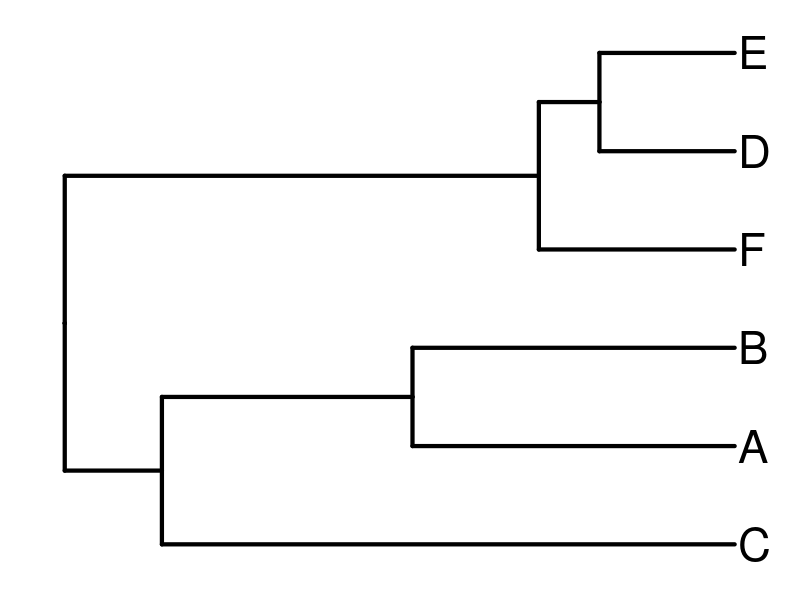
\includegraphics[width=0.4\textwidth]{phylogeny_twin.png}
  \caption{
    A phylogeny with six species
  }
  \label{fig:phylogeny}
\end{figure}

Figure \ref{fig:phylogeny} shows a phylogeny (also called 'phylogenetic tree', 
or simply 'tree') with six hypothetical species and their evolutionary 
relationships. Going from left to right, we go from the past to the present 
time. The leftmost vertical line indicates the first speciation event, called
the crown age, which gave rise to the first two ancestral species. Each
of these ancestral species gives rise to its own evolutionary history,
resulting in a tree with two clades: the ABC and the DEF clades.

Phylogenies cannot be measured directly, as they depict which species lived
when \emph{in the past}. Even with a time machine, we would have a hard time
to observe when a speciation event took place. In the present, however, we
do have species that carry their own evolutionary history with them, in the
form of DNA. 

\begin{figure}[H]
  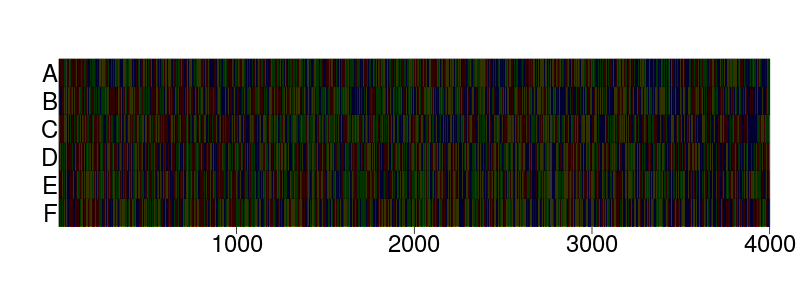
\includegraphics[width=0.8\textwidth]{alignment_twin.png}
  \caption{
    A DNA alignment of the six species
  }
  \label{fig:alignment}
\end{figure}



%\references{dissertation}

